%%%%%%%%%%%%%%%%%%%%%%%%%%%%%%%%%%%%%%%%%%%%%%%%%%%%%%%%%%%%%%%%%%%%%%%%
%    INSTITUTE OF PHYSICS PUBLISHING                                   %
%                                                                      %
%   `Preparing an article for publication in an Institute of Physics   %
%    Publishing journal using LaTeX'                                   %
%                                                                      %
%    LaTeX source code `ioplau2e.tex' used to generate `author         %
%    guidelines', the documentation explaining and demonstrating use   %
%    of the Institute of Physics Publishing LaTeX preprint files       %
%    `iopart.cls, iopart12.clo and iopart10.clo'.                      %
%                                                                      %
%    `ioplau2e.tex' itself uses LaTeX with `iopart.cls'                %
%                                                                      %
%%%%%%%%%%%%%%%%%%%%%%%%%%%%%%%%%%
%
%
% First we have a character check
%
% ! exclamation mark    " double quote  
% # hash                ` opening quote (grave)
% & ampersand           ' closing quote (acute)
% $ dollar              % percent       
% ( open parenthesis    ) close paren.  
% - hyphen              = equals sign
% | vertical bar        ~ tilde         
% @ at sign             _ underscore
% { open curly brace    } close curly   
% [ open square         ] close square bracket
% + plus sign           ; semi-colon    
% * asterisk            : colon
% < open angle bracket  > close angle   
% , comma               . full stop
% ? question mark       / forward slash 
% \ backslash           ^ circumflex
%
% ABCDEFGHIJKLMNOPQRSTUVWXYZ 
% abcdefghijklmnopqrstuvwxyz 
% 1234567890
%
%%%%%%%%%%%%%%%%%%%%%%%%%%%%%%%%%%%%%%%%%%%%%%%%%%%%%%%%%%%%%%%%%%%
%
\documentclass[12pt]{iopart}
\newcommand{\gguide}{{\it Preparing graphics for IOP Publishing journals}}
%Uncomment next line if AMS fonts required
\usepackage{iopams}  
\usepackage{graphicx}
%\usepackage{subcaption}

%\usepackage{amsmath,amssymb}
\begin{document}

\title[]{Leveraging local continuity of connected measurements for dimensionality reduction and separation of backround, signal, and noise.... }

\author{}

%%\address{IOP Publishing, Temple Circus, Temple Way, Bristol BS1 6HG, UK}
%\ead{submissions@iop.org}
%\vspace{10pt}
%\begin{indented}
%%\item[]August 2017
%\end{indented}

%\begin{abstract}
%This document describes the  preparation of an article using \LaTeXe\ and 
%\verb"iopart.cls" (the IOP Publishing \LaTeXe\ preprint class file).
%This class file is designed to help 
%authors produce preprints in a form suitable for submission to any of the
%journals listed in table~\ref{jlab1} on the next page.  You are not obliged to use this class file---we accept
%submissions using all common \LaTeX\ class and style files.  The \verb"iopart.cls"
%class file is supplied merely as a convenience for those authors who find it useful.
%This document gives both general advice that applies whatever class file you use, and specific advice
%that applies if you choose to use \verb"iopart.cls".
%
%We also accept submissions in Word format.  See elsewhere on this site for guidelines on Word submissions.
%
%If you have any queries about this document or any aspect of preparing your article for submission please contact us at the e-mail address given above.
%\end{abstract}

%
% Uncomment for keywords
%\vspace{2pc}
%\noindent{\it Keywords}: XXXXXX, YYYYYYYY, ZZZZZZZZZ
%
% Uncomment for Submitted to journal title message
%\submitto{\JPA}
%
% Uncomment if a separate title page is required
%\maketitle
% 
% For two-column output uncomment the next line and choose [10pt] rather than [12pt] in the \documentclass declaration
%\ioptwocol
%



\section{Introduction}
It is generally important in science for experimental measurements to be accompanied by uncertainties, yet it is quite common for those uncertainties--both aleatoric and epistemic--to be partially or entirely unavailable. This may be from a combination of factors: e.g. poorly characterized backgrounds, lack of sufficient models for detector characteristics, and stochastic variations in properties of the observed system itself that are unrelated to the physics of interest yet confound the analysis. At the same time, there may be significant reduncancy across measurements with respect to the underlying signal.

Diffraction and spectroscopy experiments undertaken at synchrotron and XFEL light sources are an example of such a setting: they generate large volumes of data that are rich in information but plagued by contributions such as shot noise, beam energy and intensity jitter, sample nonuniformity and detector artifacts. However there is often an intrinsic connectedness between successive measurements taken on a progression of different physical states: for example, values of the state variables in a thermodynamic study. There may also be further data redundancy, as many methods--such as powder diffraction and serial crystallography--require repeated measurements of the same system to accumulate sufficient statistics or orientational averaging. Consequently, large spectroscopic or diffraction datasets generated at third- or fourth-generation light sources are likely to contain sequences of measurements that combine smooth variation with respect to underlying physical parameters with a uncertainty whose underlying distribution is \emph{a prior} unknown but that is discontinuous and substantially uncorrelated from one measurement to the next. 
 %Define ordered and connected

Taking a series of 1d measurements, the relevant underlying physical parameters can be treated as ordinal variables to the dataset into a tensor of the form 

\begin{equation}
X_{i_1i_2...i_N, iq}
\end{equation}

where the first $i_1$ to $i_N$ index the ordinal variables and $iq$ indexes the 1d measurement grid ($q$ denotes momentum transfer in 1d x-ray diffraction, which for concreteness we will assume is the experimental modality).

%for which each distinct sequence of values for the indices $i_1, i_2,...
%i_N$ corresponds to a single spectrum or diffraction pattern, $q$
%indexes momentum transfer or energy in the case of XRD or spectroscopy,
%respectively, and each of the indices $i_n, n \in \{1, 2, ... N\}$
%corresponds to an ordering dimension along which direction the
%underlying signal's variation is smooth. The dimensionality of the
%dataset is thus simply one higher than $N$, the number of ordinal
%attributes.
%

The connectedness of $X$ with respect to indices $i_1, i_2, ... i_N$ describes both the sample-derived signal and any smoothly-varying
background. We label the signal and stochastic components of $X$ as $S$ and $\eta$, respectively: $X = S + \eta$.
 
%#other contributions to the measured X-ray
%#intensity--such as shot noise, one-off artifacts, and stochastic
%#variations across different portions of the sample--are independent or
%#at least substantially stochastic. We label the signal and stochastic components of $X$ as $S$ and $\eta$, respectively: $X = S + \eta$. 

\emph{elaborate that, if the dataset is underssampled. $\eta$ is not entirely a result of statistical uncertainty; i.e. it also includes epistemic uncertainty}

In the particular setting of powder diffraction analysis one can additionally exploit other prior information about the data: for example, the signal is concentrated in peaks that are narrow in $q$-space, which allows further separation of $S$ into crystalline and diffuse diffraction components.


In this work we present an approach for separating connected
measurements into their components $S$ and $\eta$. We then apply this
separation method to two germane x-ray diffraction analyses: (1) robust
identification of powder diffraction peaks and (2) a feature extraction
method for combinatorial materials discovery datasets that addresses the
problem of peak-shifting, a long-standing impediment to the automated
reconstruction of phase diagrams in the field of high-throughput
materials discovery. To demonstrate the method's robustness and generalization we
consider cases in which the space of measurement conditions are one- and
two-dimensional: respectively, a temperature study of xxxx material and
a combinatorial study of the CoNiTi ternary system.

These results suggest that handling connected datasets in the proposed fashion
brings two types of benefits: (1) we get simple signal-to-uncertainty
heuristics that allow more principled modeling and interpretation of
measurements, and (2) prior physical information becomes captured in
geometry, since Euclidean distance between sites in the data tensor $X$
has a direct relation to distance in physical parameter space.

\emph{there's probably a better way of saying this. and probably fits better in the abstract or conclusion.}
\emph{maybe elaborate on item (1), mentioning its importance to (2) and any other downstream analysis where one would want to use signal-to-noise heuristics.}
%(note: high-frequency variation is a
%more accurate description here, uncorrelated is a limiting case but it
%simplifies the interpretation).

%In particular, we consider two XRD datasets--a %--to demonstrate the separation of connected data into
%a physically relevant component and a component that comprises
%noise and artifacts. 
%We represent this as sepration of the signal into two components: $X = \hat{X} + \eta$, where
%$\hat{X}$ is slow-varying in the ordinal dimensions and $\eta$ is a fast-varying noise
%contribution (again, in the ordinal dimensions). The approach depends only on the minimal assumption of
%connectedness and so should be applicable, with minor tuning, to any
%dataset.


% In section xxxx we show a feature extraction scheme for XRD
%phase mapping datasets that is based on local connectivity. The approach
%is robust to peak-shifting, which until now has been long-standing
%frustration for the interpretation of such datasets.
\emph{say why this is new and good, motivate and compare to prior efforts in the community}

%use  connectedness of measurements to separate a collection of spectral or diffraction
%
%In this paper we consider ways in which the redundancy of datasets connected by 
%
%This redundancy, we argue, creates an opportunity to use the mutual information accross different measurements to make.... information... robust or whaterver.... 
%
%Rich in information, plagued by noise and artifacts. 
%
%IN the paper, we want to show how we can leverage the connectedness of the measurements ... yada yadaa minimal assumptions, separate useful information from these large datasets.
%
%1. LS collect connected datasets
%2. rich in information but also artifacts and noise (background, peak shifting artifact, noise)
%    2. a Introduce Yijin and Suchi's data
%3. leveraging connectedness, we can separate these datasets. -> expand into the body of the paper.
%    3. a Define connectedness, state assumptions. Good measurements oversample the measrement space. We can use this oversampling to help separate datasets into different components with minimal assumptions. Connect 
%(work on the title)

%## Introduction
%* aim for JSR? large facilities (synchrotron, XFEL) produce large connected datasets (cites). 
%* Neighborhood and continuity can be exploited in two ways: to estimate noise (in the absence of a noise model) and to extract features. 
%* Motivating applications: combi; any 'dense' dataset over a range of values for the key experimental parameter.
%* Motivating problem: peak shifting is difficult to model; naive similarity metrics are not robust to it. What's the most parsimonious way of grouping XRD patterns for structures that are the same up to lattice parameter distortions? We will show that continuity + neighborhood is sufficient.
%* Discuss, cite prior literature

\section{Methods}

\subsection{Prior approaches}
Summarize approaches using simple similarity measures, such as cosine distance in the diffraction space.

\begin{figure}
  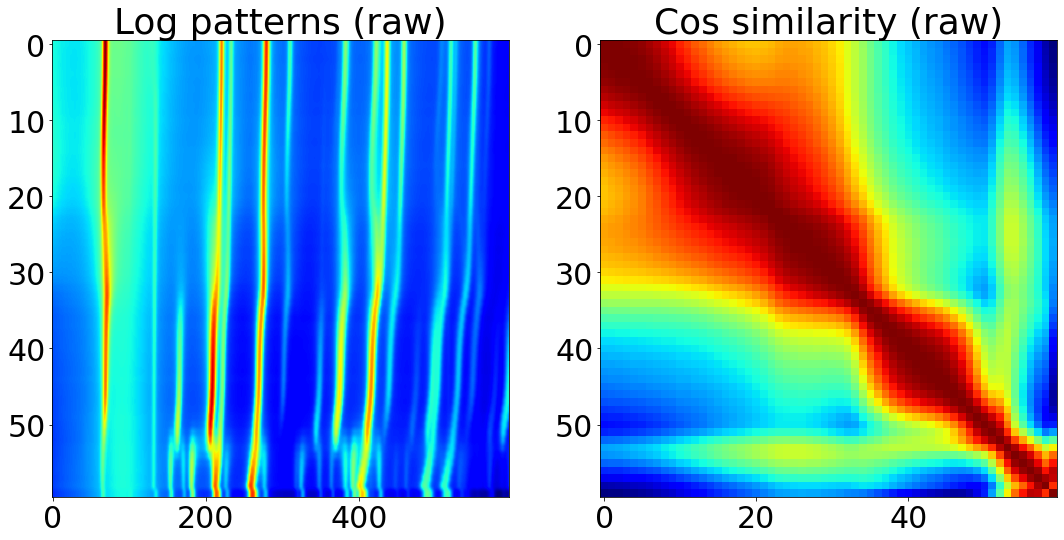
\includegraphics[width=\linewidth]{paper_figures/1/raw_with_similarity.png}
  \caption{(a) Heatmap of 60 experimental diffraction patterns of the XXX system at diffferent temperatures, ordered vertically in decreasing temperature. (b) Heatmap of cosine similarity between pairs of those diffraction patterns (a)}
  \label{fig:noise}
\end{figure}

\begin{figure}
  %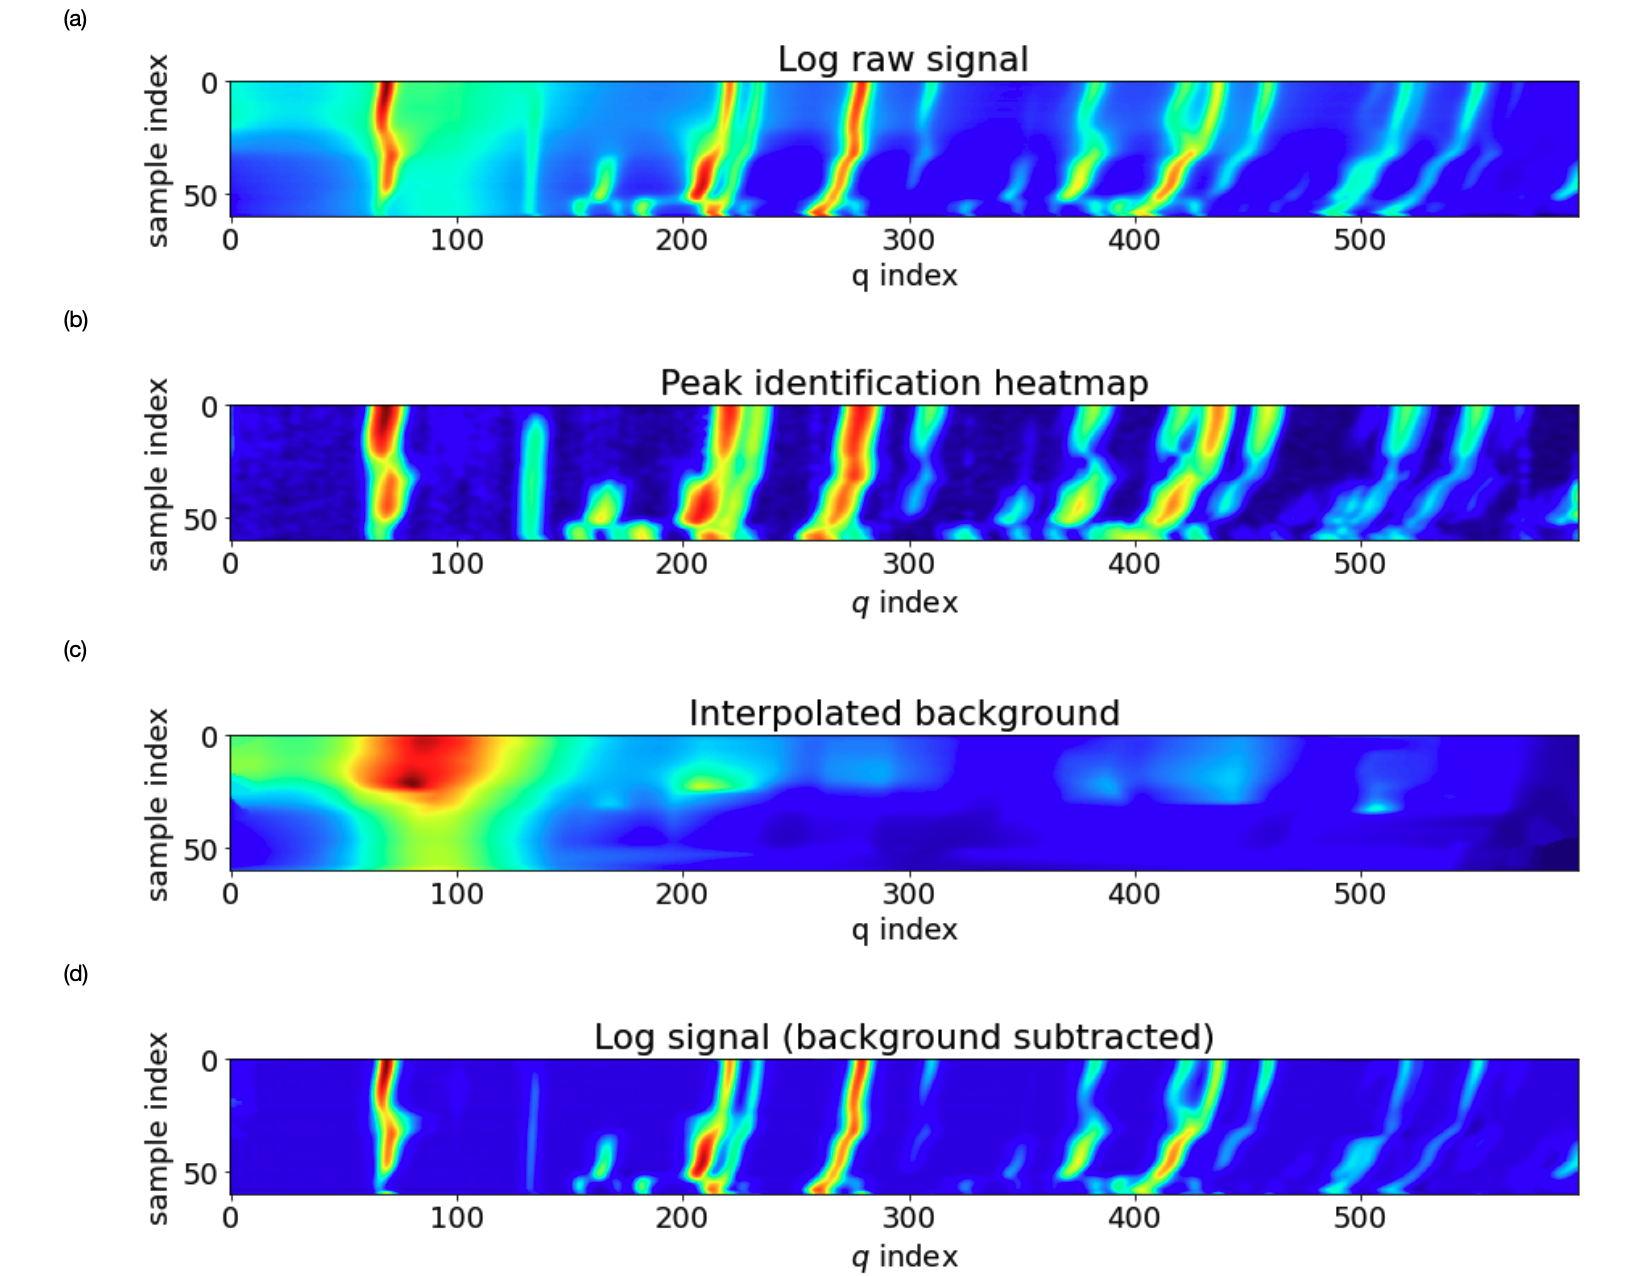
\includegraphics[width=\linewidth]{figures/heatmaps.png}
  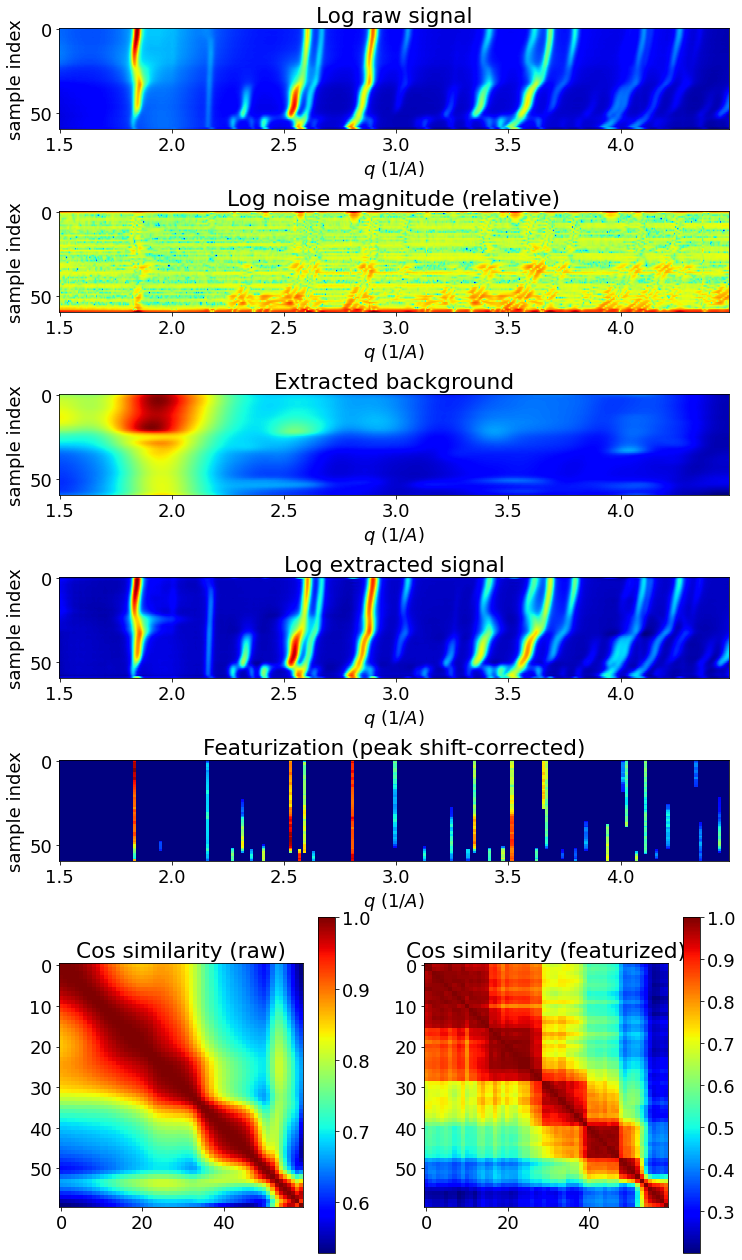
\includegraphics[scale=.5]{paper_figures/pkg/2_T_summary.png}
  \caption{ (a) Heatmap of XRD dataset $X_{iq}$ corresponding to a temperature scan
of XRD patterns for xxxxx system. The vertical index $i$ and horizontal
index $q$ index temperature and momentum transfer, respectively. }
  \label{fig:heatmaps}
\end{figure}
%Separation: either fast/slow or frequency-based variation. Frequency of variation is the key idea. 
%
%Alternative: median / quartile variation based on population density. Acknowledge these alternatives. 
%
%Consider cost of computation: what's the method that would allow an event-detection-type setup. See if we could sell this type of thing to the detector group at SLAC that works on ASICS for rare evetns. 
\subsection{Background subtraction}
The first step to estimating the background is to identify the peak
regions, which must be excluded before calculating the background. In
the case of typical diffraction data a simple high-pass DFT filter does
not cleanly extract the peaks when phase is retained in the inverse
Fourier transform. This is because of the presence of ringing artifacts
as well as the high concentration of signal in the diffraction peaks,
which pile on top of the background in the low-frequency region of the
power spectral density. On the other hand we can identify peak regions
with the following transformation:

%by padding the signal in the $q$ dimension, taking a 1D DFT, and
%suppressing low-frequency components with a simple filter:

% TODO effect of zero-padding / extrapolation
\begin{equation}
N(0, \sigma) \circledast |{F}^{-1}(H  {F}(q))|,
\end{equation}

where $N$ is a unit Gaussian in q with standard deviation $\sigma$
is chosen to match the diffraction peak width, $\circledast$ denotes
convolution, $F$ denotes Fourier transformation and $H$ is a Blackman window.

\emph{this part will be fleshed out. some steps are still omitted}

The background is then estimated by smoothed nearest-neighbor interpolation in multiple dimensions, wherein data from non-peak regions is used to
fill in background intensities within the peak regions (Fig. 1(c)). An adjustable threshold parameter $t$ specifies the fraction of pixels belonging to peak regions; favorable values of $t$ depend mainly on the noise level and density of diffraction peaks in a particular dataset, and are determined manually. 
Finally, the background estimate is subtracted from the denoised data (Fig. 1(d)).

To make for a simple extension to datasets of arbitrary dimensions we
estimate the background by linear interpolation in the q dimension
alone, together with a N-dimensional nearest-neighbor assignment to
fill in points out of range for interpolation.

\subsection{Noise estimation}
%\begin{figure}
%  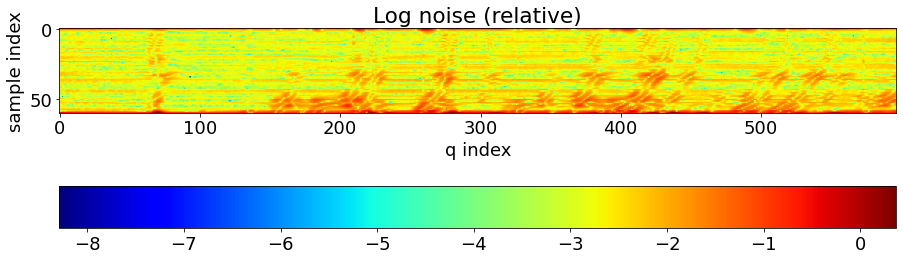
\includegraphics[width=\linewidth]{figures/noise.png}
%  \caption{}
%  \label{fig:noise}
%\end{figure}
While in the case of intensity variation in the q dimension we assume
that high-frequency features belong to the informative (i.e. physical)
component of the signal, in the case of the ordering dimensions we
make the opposite assumption that the physically relevant part of the
signal varies smoothly from one XRD pattern to any adjacent one, while
any high-frequency, uncorrelated deviations from this progression are
due to either noise (from e.g. detector characteristics or Poisson
statistics) or artifacts (such as insufficient orientational sampling
of the diffracting crystallites). Under this assumption the signal and
noise lack substantial overlap in the N-1-dimensional Fourier transform
along ordering dimensions; thus we can use a simple DFT filter to
separate them (Fig. 2)

The above estimations of background and noise components separate
the signal into estimates of the signal component $S$ (which in turn separates into
background + diffuse scattering and diffraction) and uncertainty values
that are interpreted as single samples of an unknown underlying noise distributions. Despite its poorly-characterized nature, the latter of these can be used to propagate uncertainties to any downstream analyses. 

We label the signal and background $\hat{S}$ and $B$, respectively,
so that $X = \hat{S} + B + \eta$.

\emph{some discussion is needed on the difference in interpretation of the noise estimate in undersampled vs. sufficiently sampled datasets}

\section{Methods and Discussion}
\subsection{Application: feature extraction}
The above analysis addresses the data itself, with no scientific
interpretation aside from the separation between crystalline and diffuse
contributions to the scattering signal. However, we find that the same
ordering and smoothness properties are useful for reducing the data into
salient \emph{information}, where the goal is to find physically-meaningful
boundaries in the ordering dimensions corresponding to, e.g., the
surface separating a single-phase region from surrounding multi-phase
regions in a combinatorial diffraction dataset. Specifically, we 
identify diffraction peaks in every XRD pattern, independently, and then
link each peak in a pattern to any q-adjacent peaks in neighboring patterns (i.e. patterns that are adjacent in $i_1, i_2 ... i_N$). 

Each contiguous set of peaks linked in this way is denoted as a feature, and the ensemble of features defines a new representation of the dataset $ Y_{i_1,i_2...i_N, j} $, where $j$ indexes the peak features. The entries of $Y$ are 0 where the corresponding pattern lacks feature $j$, and equal to the intensity of the feature-peak combination otherwise.

Peak parameters are obtained using a curve-fitting procedure that relies on Scargle's Bayesian Block algorithm to segment each 1d measurement into signal regions (i.e. blocks) and then performs iterative peak-fitting on every block through a nonlinear least squares optimization on a sum of peak profiles. A Voigt profile is used in this work as it is appropriate for powder diffraction data. 

For an individual block comprised by a set $B$ of momentum transfers, peak profiles are added to the fit curve until the fit residual $R$ satisfies

\begin{equation}
(\Sigma_{q \in B}\frac{1}{N}\frac{R_q^2}{\eta_{q}^2}))^{1 / 2}  < s,
%|R \oslash \eta|
\end{equation}

where $s$ is a threshold parameter of order unity.% and $\oslash$ denotes elementwise division.

\emph{cover the utility of noise estimates and background subtraction for better peak fitting}


\begin{figure}
  \centering
  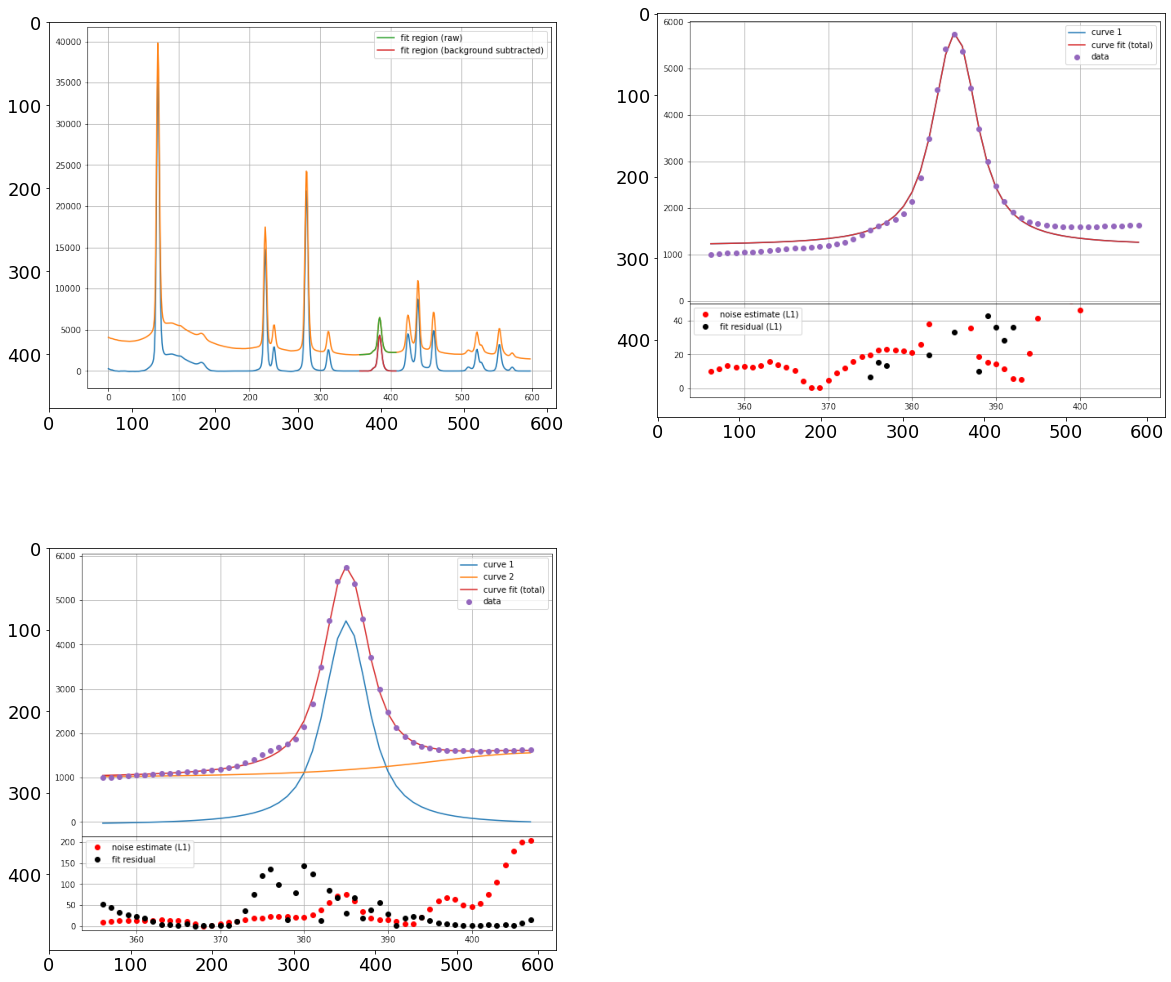
\includegraphics[scale=0.5]{paper_figures/pkg/3_BBA.png}
  \caption{(a) Powder diffraction pattern of the xxx system showing background subtraction and a single Bayesian block in red. (b) Iterative peak fitting of the single block using estimated noise relative to curve fit residual to determine the number of peak profiles to include. 

\emph{This figure needs to be
 reformatted (font size, layout). I will add a third panel showing the effect of background subtraction on the number of peak profiles found.}}
  \label{fig:features}
\end{figure}

%utility of this is that it removes peak-shifting,
%etc….

\begin{figure}
  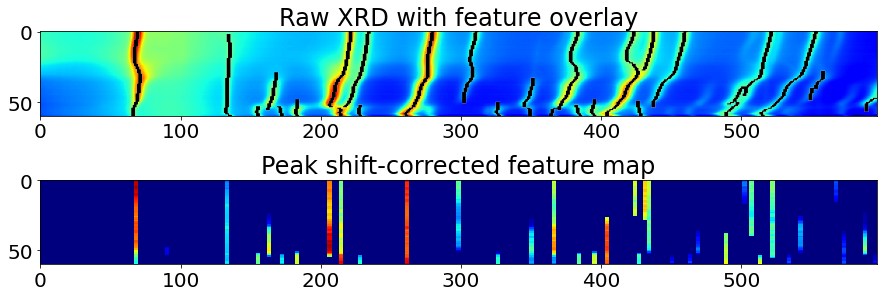
\includegraphics[width=\linewidth]{paper_figures/pkg/4_Tfeatures.png}
  \caption{(a) Features identified from peaks connected in
$i,q$ space for XRD dataset $X_{iq}$ corresponding to a temperature scan
of XRD patterns for xxxxxx system. Index $i$ denotes temperature.
    
(b) Intensity profile along each of the features in (a).}
  \label{fig:features}
\end{figure}

\begin{figure}
  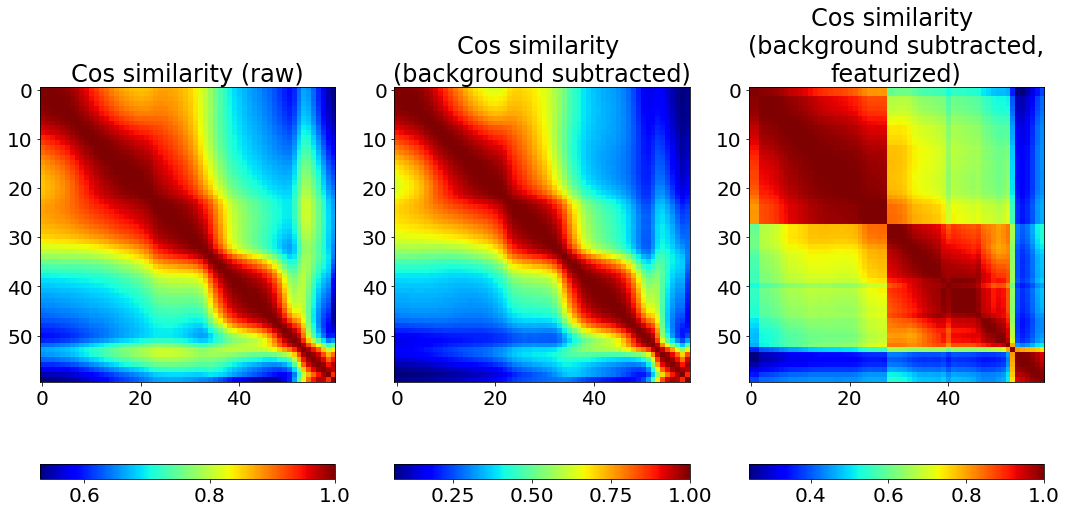
\includegraphics[width=\linewidth]{paper_figures/pkg/5_T_peakfit.png}
\caption{Comparison of cosine similarity squares for (a) raw powder diffraction of the xxx system, (b) post background
 subtraction, and (c) peak shift-corrected feature vectors derived from the same dataset.
}
  \label{fig:simsquares}
\end{figure}

\begin{figure}[h!]
  \centering
%  \begin{subfigure}[b]{0.4\linewidth}
    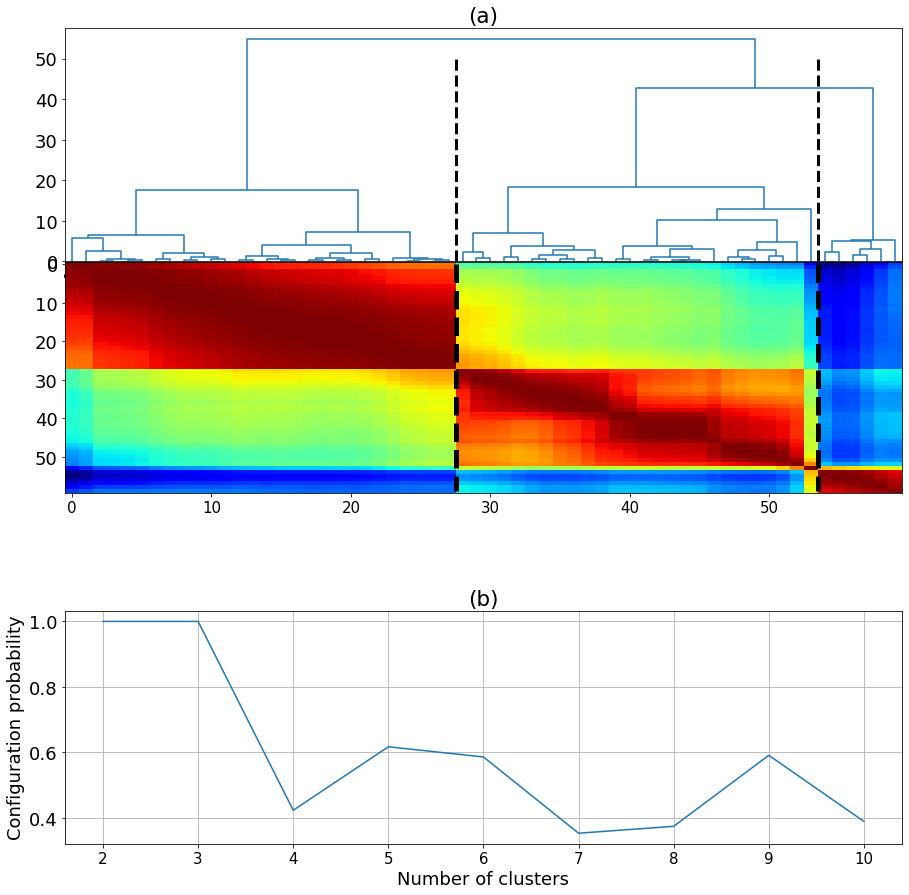
\includegraphics[scale = .55]{paper_figures/pkg/8_Tclustering.png}
%    \caption{(a)}
%  \end{subfigure}
%  \begin{subfigure}[b]{0.4\linewidth}
%    \caption{(b)}
%  \end{subfigure}
  \caption{(a) Optimal clustering for a set of XRD patterns demonstrating a
temperature progression in xxxx system. The optimal number of clusters
is determined by clustering stability over an ensemble of XRD patterns
generated by draws from a according to the simple noise model described in section xxxx.

(b) Ensemble probability of the most probable cluster configuration
for agglomerative clustering with Ward linkage criterion, for the same
dataset. Horizontal axis varies the number of clusters.
}
  \label{fig:7}
\end{figure}

\begin{figure}[h!]
  \centering
%  \begin{subfigure}[b]{0.4\linewidth}
%    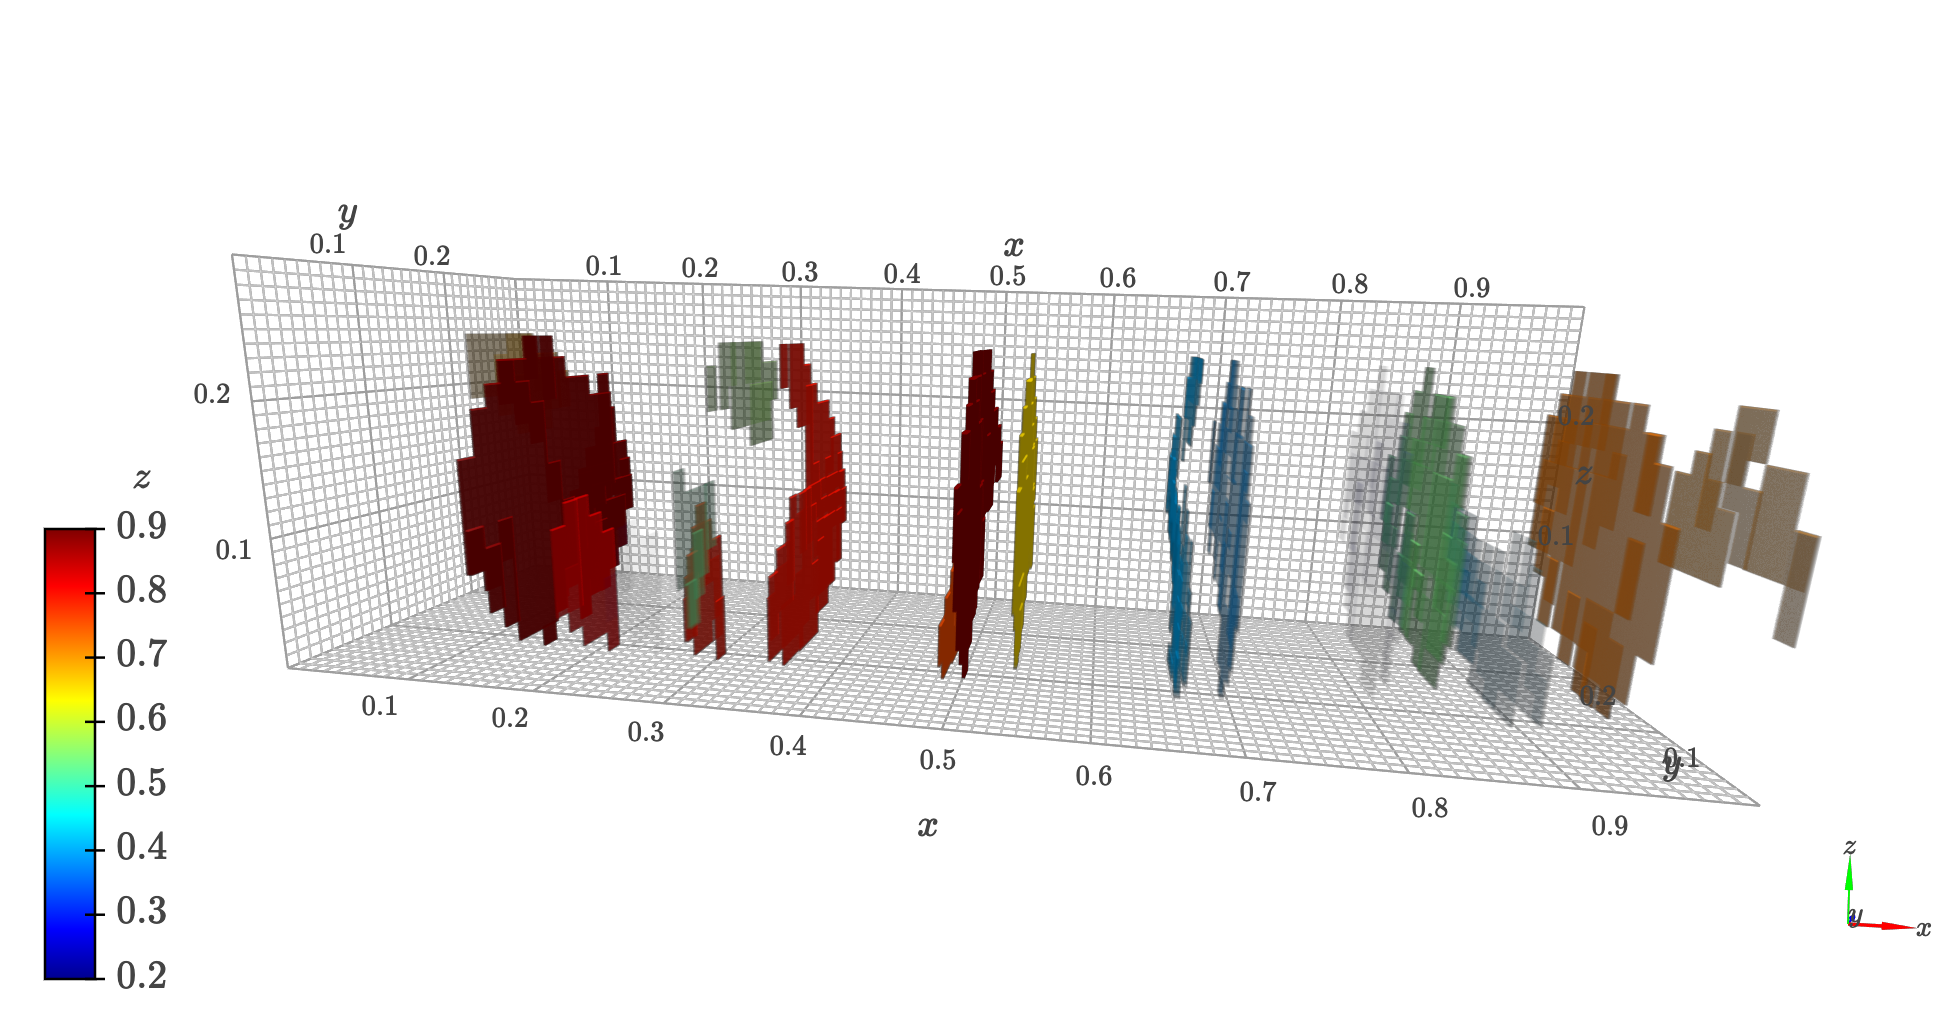
\includegraphics[width=\linewidth]{figures/3d_features.png}
%    \caption{(a)}
%  \end{subfigure}
%  \begin{subfigure}[b]{0.4\linewidth}
    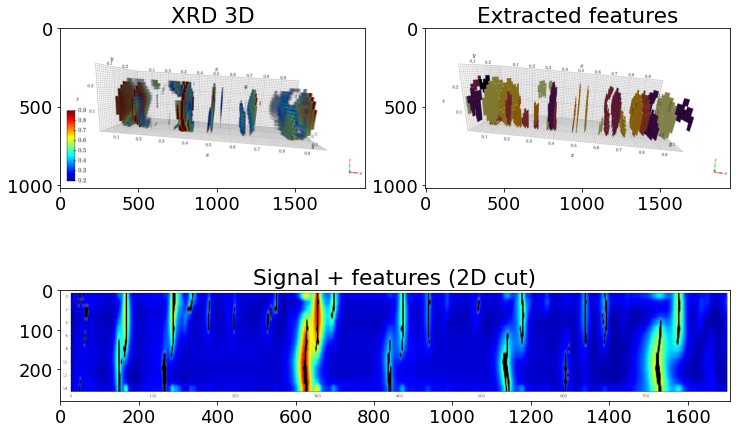
\includegraphics[width=\linewidth]{paper_figures/pkg/6.png}
%    \caption{(b)}
%  \end{subfigure}
  \caption{(a) volumetric heatmap for a three-dimensional diffraction study of the CoNiTi ternary system. Dimensions x any y are coordinates on the compositional simplex, while dimension z indexes momentum transfer. (b) Three-dimensional rendering of peak features identified by the shift-correcting procedure described in section xx. (c) Two-dimensional cut of the dataset displayed in (a), with peak features overlayed in black.}
  \label{fig:6}
\end{figure}

\section{Supplemental figures}
\begin{figure}[h!]
  \centering
%  \begin{subfigure}[b]{0.4\linewidth}
    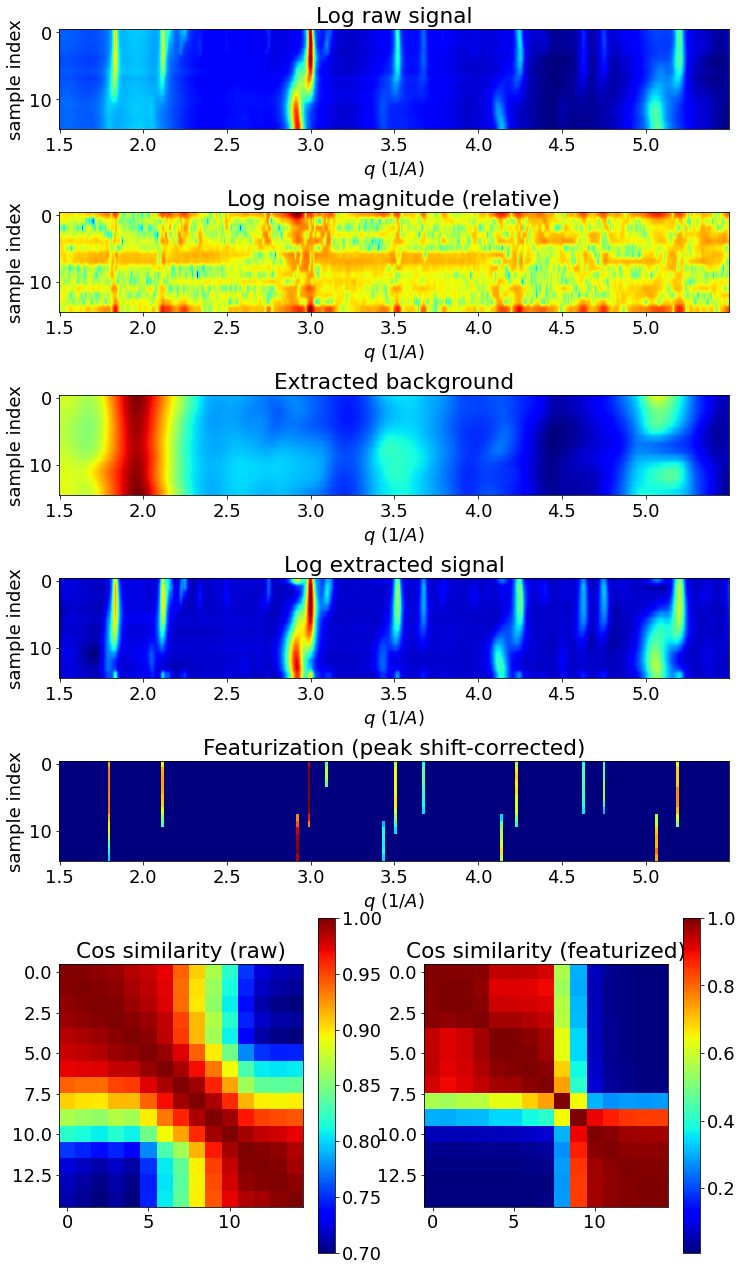
\includegraphics[scale = .5]{paper_figures/pkg/7_composition_summary_peakfit.png}
%    \caption{(a)}
%  \end{subfigure}
%  \begin{subfigure}[b]{0.4\linewidth}
%    \caption{(b)}
%  \end{subfigure}
  \caption{Separation and feature extraction for a 2d slice of the CoNiTi ternary system.}
  \label{fig:7}
\end{figure}

%* Discuss caveats: some features are broken up, others are merged. Since there's typically plenty of reduncancy due to the multiple lines that appear with each phase, we think that the feature extraction is robust to these errors.
%* Further interpretation: this is a dimensionality reduction technique. Not a scientific methodology in itself (i.e. the extracted information still has to be interpreted), but a possible improvment over prior methods that are very fragile with respect to peak shifts. 

\section{Conclusions and future work}

In this section, we propose using this type of approach for event detection in a high-data rate environment. We can also talk about the prospect that our peak shift-correction will help solve the phase-mapping problem.


\section{References}

\end{document}
